\subsection{Expectation propagation}
\label{sec:chap2_ep_algorithm}

Now we consider a distribution $p(\bm{\theta}) \propto \prod_{a} \tilde{f}_a(\bm{\theta}_a)$, where $\tilde{f}_a$ are the factors in the corresponding factor graph with associated variables $\bm{\theta}_a$. A prevalent example for such a distribution is the exact posterior, where now $\tilde{f}_a$ represents either the prior distribution or the likelihood function associated with a datum. The marginal probability of a subset of $\bm{\theta}$ can be complicated. The highly successful Expectation Propagation (EP) \citep{minka:ep2001} algorithm approximates these exact marginals by another factor graph with a collection of simpler functions $q(\bm{\theta}) \propto \prod_{a} f_a(\bm{\theta}_a)$. It iteratively updates the approximating factors $\tilde{f}_a$ through the ``exclusion-moment matching-inclusion'' procedure, detailed in Algorithm \ref{alg:ep_general}.

%
To summarise the algorithm, we first define the ``leave-one-out'', or \emph{cavity distribution}\footnote{The name ``cavity'' comes from the \emph{cavity method} that is used to study Ising models \citep{mezard:spin1987}, again showing the deep connections between EP and belief propagation.}
\begin{equation}
q_{-a} \propto \prod_{b \neq a} f_b(\bm{\theta}_b) \propto q(\bm{\theta}) / f_a(\bm{\theta}_a),  
\end{equation}
which is computed by multiplying all the other factors except the selected one. Also an ordering of this factor selection is called a \emph{schedule} of the EP algorithm, and in the following we assume it is random. The second step is to compute the \emph{tilted distribution} by inserting back the true factor $\tilde{f}_a$ that $f_a$ approximates:
\begin{equation}
\tilde{p}_{a}(\bm{\theta}) \propto q_{-a}(\bm{\theta}) \tilde{f}_a(\bm{\theta}_a),
\end{equation}
and update the selected factor $f_a$ by minimising the KL divergence from $\tilde{p}_{a}$ to the approximation $q$ (with $f_a$ included), with the restriction that the new $q$ belongs to the same family of previous approximation. For exponential family approximations, we solve this optimisation problem by zeroing the gradients of the KL w.r.t.~the natural parameters of $q$. This is equivalent to matching the moments of the arguments between the two distributions. More precisely, assume the factors $f_a$ belong to the same exponential family with feature function $\bm{\Phi}(\bm{\theta}) = (\Phi_1(\bm{\theta}), ..., \Phi_d(\bm{\theta}))$, then we write the $q$ distribution as
\begin{equation}
q(\bm{\theta}) \propto \exp(\bm{\lambda}^{\text{T}} \bm{\Phi}(\bm{\theta})),
\label{eq:chap2_ep_expfam_param}
\end{equation}
where $\bm{\lambda}$ denote the natural parameters. Zeroing the gradient of $\mathrm{KL}[\tilde{p}_{a} || q]$ wrt.~$\bm{\lambda}$ (and viewing $\tilde{p}_{a}$ as constant) returns
\begin{equation}
\mathbb{E}_{q} \left[ \bm{\Phi}(\bm{\theta}) \right] = \mathbb{E}_{\tilde{p}_{a}} \left[ \bm{\Phi}(\bm{\theta}) \right],
\label{eq:chap2_ep_moment_matching}
\end{equation}
%
which gives the name of moment matching \citep{seeger:ep2005}. We denote this optimisation computation with $\mathrm{proj}$ operator
\begin{equation}
\mathrm{proj}[p] = \arg\min_{q} \mathrm{KL}[p|| q],
\end{equation}
which returns the minimiser of the KL-divergence $\mathrm{KL}[\tilde{p}_{a}||q]$ by passing the moments of $\tilde{p}_{a}$. This operator is also called M-projection \citep{cover:itbook1991}. After the computation of $q^* = \mathrm{proj}[\tilde{p}_a]$ we recover the update of $f_a$ by
\begin{equation}
f_a(\bm{\theta}_a) \leftarrow q^*(\bm{\theta}) / q_{-a}(\bm{\theta}).
\end{equation}
%
To improve convergence damping updates can be applied to step 4 in Algorithm \ref{alg:ep_general} as
\begin{equation}
f_a(\bm{\theta}_a) \leftarrow f_a(\bm{\theta}_{a})^{1 - \epsilon} \left(\mathrm{proj}[\tilde{p}_{a}] / q_{-a}(\bm{\theta}) \right)^{\epsilon},
\end{equation}
where $\epsilon$ denotes the step-size. The last step, corresponded to the inclusion step in Algorithm \ref{alg:ep_general}, is to incorporate the updated factor back to the approximation:
\begin{equation}
q(\bm{\theta}) \leftarrow q_{-a}(\bm{\theta}) f_a(\bm{\theta}_a).
\end{equation}
The reader may find that in Algorithm \ref{alg:ep_general} the updated distribution $q$ equals to $q^*$ in the moment matching step, while this yields EP without damping only.

%
\begin{algorithm}[t] 
\caption{Expectation Propagation (without damping)} 
\label{alg:ep_general} 
\begin{algorithmic}[1] 
%\STATE initialize $\{\tilde{f}_a\}$
\WHILE{not converged}
	\STATE choose a factor $f_a(\mparam_a)$ to refine (according to a schedule):
	\STATE exclusion: $q_{-a}(\bm{\theta}) \propto q(\bm{\theta}) / f_a(\bm{\theta}_a)$
	\STATE moment matching: $f_a(\bm{\theta}_a) \leftarrow \mathrm{proj}[q_{-a}(\bm{\theta}) \tilde{f}_a(\bm{\theta}_a)] / q_{-a}(\bm{\theta})$
	\STATE inclusion: $q(\bm{\theta}) \leftarrow q_{-a}(\bm{\theta}) f_a(\bm{\theta}_a)$
\ENDWHILE
%\RETURN $\{\tilde{f}_a\}$
\end{algorithmic}
\end{algorithm}
%


\vspace{1em}
\begin{tcolorbox}
\textbf{Remark} (misconceptions about EP)\textbf{.}
A misleading interpretation states that EP is the counterpart algorithm of VI which minimises the inclusive KL. The correct answer is more than ``yes or no'' and it strongly depends on the factor graph structure.
If the factor graph only contains a single factor node, then EP is minimising the inclusive KL globally. However, computing moments on this factor graph often requires further approximations, thus it is rarely considered in EP literature until the development of Chapter \ref{sec:vrbound_all}. Otherwise, EP does \emph{not} minimise the inclusive KL divergence to the target distribution. Thus we refer EP as a \emph{local approximation} algorithm since it works with the components of the target distribution directly. Conversely, VI does minimise the exclusive KL divergence \emph{globally}, regardless of the factor graph structure.
\end{tcolorbox}

\subsubsection{Why EP works}
%(how to describe the intuition well?)\\
In general, to obtain an accurate approximation for some complicated distribution is a difficult task, as estimating the approximate functions \textit{jointly} is often intractable. Factor graphs provide not only a factorised representation of the true distribution but also a guide for choosing the function families for approximation. Consider the minimisation task $q^* = \argmin_q \mathrm{D}[p || q]$.\footnote{Here the measurement can be any distance or divergence, each returns different benefits. In EP the divergence measure is the KL divergence.} Below we discuss 3 difference methods for the optimisation problem, where we understand them as different schedules.\footnote{This is an explanatory discussion rewritten from my first year report.}

The simplest way is independent factorised approximation, i.e.~to approximate each factor independently. This returns a fast and parallelisable algorithm that a simple map-reduce scheme can be applied to. However, is it common that factors share random variables, in which the marginals of the selected factor's random variables can deviate from that factor's function value. From the nature of product we know that small errors of each factor approximation can easily accumulate to large errors of the final result $q$. 

The statistics and control communities have noted the importance of including the dependence in approximation, resulting in the well-known assumed density filtering (ADF) algorithm \citep{maybeck:adf1982}. It can be viewed as a restricted version of factorised approximation by greedily adding in more factors to the $q$ distribution such that $q(\mparam) f_a(\mparam)$ matches $q(\mparam) \tilde{f}_a(\mparam)$ as close as possible. One simple example would be approximating $p(\mparam) = \tilde{f}_1(\mparam) \tilde{f}_2(\mparam) \tilde{f}_3(\mparam)$ with $q(\mparam) = f_1(\mparam) f_2(\mparam) f_3(\mparam)$. Assume we start from an accurate estimation of $f_1(\mparam) \approx \tilde{f}_1(\mparam)$ (where now $q(\mparam) = f_1(\mparam)$), ADF in current iteration incorporates $f_2(\mparam)$ (or $f_3(\mparam)$ depending on the schedule) to the $q$ distribution, updates $f_2(\mparam)$ such that it minimises $\mathrm{D}[q(\mparam) \tilde{f}_2(\mparam) || q(\mparam) f_2(\mparam)]$,
and includes the new approximation $f_2(\mparam)$ to the new $q(\mparam) \leftarrow f_1(\mparam) f_2(\mparam)$. 
The disadvantage of this approach is its sensitivity to the choice of the schedule, especially when a subset of variables is shared by most of the factors. 

EP tries to address the problem of sensitivity to scheduling by looping through the factors repeatedly, giving a chance for inaccurate factors to ``correct themselves''. This puts further restrictions to the mean-field update by including all the factors in moment matching. The precision may oscillate as the approximation in the first few loops can be very poor, especially considering EP is reduced to ADF in the first iteration if initialising all the approximating factors as 1 (which is often the case). Also there is no guarantee for EP to converge. But EP (and in general message passing) is still an efficient algorithm, especially when applying to only a subset of factors (see the application to error-correcting codes \citep{peterson:ecc1972} and TrueSkill algorithm \citep{herbrich:trueskill2006}). 

\subsubsection{Linking power EP and $\alpha$-divergence}
An extension of EP is power EP \citep{minka:powerep2004}, which excludes a fraction of the approximation (i.e. $f_a(\bm{\theta})^{\alpha}$) and includes the same fraction of the true factor for updates (see Algorithm \ref{alg:powerep_general}). Since we exclude/include only a fraction of the factors, damping should be applied to the natural parameters of $f_a(\bm{\theta})^{\alpha}$ directly before recovering the update for $f_a(\mparam)$.

\begin{algorithm}[t] 
\caption{Power EP with fraction $\alpha$} 
\label{alg:powerep_general} 
\begin{algorithmic}[1] 
%\STATE initialize $\{\tilde{f}_a\}$
\WHILE{not converged}
	\STATE choose a factor $f_a(\mparam_a)$ to refine:
	\STATE exclusion: $q_{-a}(\bm{\theta}) = q(\bm{\theta}) / f_a(\bm{\theta}_a)^{\alpha}$
	\STATE moment matching: $f_a(\bm{\theta}_a)^{\alpha} \leftarrow \mathrm{proj}[q_{-a}(\bm{\theta}) \tilde{f}_a(\bm{\theta}_a)^{\alpha}] / q_{-a}(\bm{\theta})$
	\STATE inclusion: $q(\bm{\theta}) \leftarrow q(\bm{\theta}) f_a(\bm{\theta}_a) / f_a(\bm{\theta}_a)^{old}$
\ENDWHILE
%\RETURN $\{\tilde{f}_a\}$
\end{algorithmic}
\end{algorithm}

Power EP with fraction $\alpha$ corresponds to minimising the $\alpha$-divergence from $\tilde{p}_{a}(\mparam) \propto q(\mparam) \tilde{f}_a(\mparam) / f_a(\mparam)$ to $q(\mparam)$. To see this, we first adapt Amari's definition \citep{amari:ig1985} of $\alpha$-divergence $\mathrm{D}_{\alpha}^{A}$ to the following form \citep{zhu:divergence1995, minka:divergence2005}, which we refer to as Minka's $\alpha$-divergence:
\begin{equation}
 \mathrm{D}_{\alpha}^{M}[p||q] = \frac{1}{\alpha (1 - \alpha)} \left( 1 - \int p(\bm{\theta})^{\alpha} q(\bm{\theta})^{1 - \alpha} d\bm{\theta}\right)\,
\end{equation}
which is equivalent to the original definition by setting $\alpha' = 2 \alpha - 1$ in Amari's notation $\mathrm{D}_{\alpha'}^A = \mathrm{D}_{\alpha}^M$.
%
So similarly the exclusive KL divergence $\mathrm{KL}[q || p] = \lim_{\alpha \rightarrow 0} \mathrm{D}_{\alpha}^M [p || q]$ and the inclusive one $\mathrm{KL}[p || q] = \lim_{\alpha \rightarrow 1} \mathrm{D}_{\alpha}^M [p || q]$ can be recovered. Now we investigate the case which replaces the moment matching step in the EP algorithm (Algorithm \ref{alg:ep_general}) by $q^* = \argmin D_{\alpha}^M[\tilde{p}_{a}||q]$, which is also called $\alpha$-projection \citep{amari:ig2000}. Similarly we assume $q$ has an exponential family form (\ref{eq:chap2_ep_expfam_param}), and we fix $\tilde{p}_{a}(\mparam)$ as the target. Then when $\alpha \neq 0, 1$,
\begin{equation*}
\begin{aligned}
\nabla_{\bm{\lambda}} D_{\alpha}^M[\tilde{p}_{a}||q] &= \frac{1}{\alpha} \left( \mathbb{E}_{q}[\bm{\Phi}(\bm{\theta})] - \mathbb{E}_{\tilde{p}_{a}^{(\alpha)}}[\bm{\Phi}(\bm{\theta})] \right), \\
\tilde{p}_{a}^{(\alpha)} &\propto \tilde{p}_a^{\alpha} q^{1 - \alpha}.
\end{aligned}
\end{equation*}
In this case the solution of $\nabla_{\bm{\lambda}} D_{\alpha}^M[\tilde{p}_{a}||q]$ is non-trivial since now $\tilde{p}_{a}^{(\alpha)}$ contains contributions from $q$. Instead power EP proposes a fixed point iterative update procedure, by initialising $q$ with last iteration's solution (which makes $\tilde{p}_{a}^{(\alpha)} \propto q \tilde{f}_a^{\alpha} / f_a^{\alpha}$, see the moment matching step in Algorithm \ref{alg:powerep_general}), fixing $\tilde{p}_{a}^{(\alpha)}$ as the target, and computing the next update for the natural parameter $\bm{\lambda}$ such that the moments of $q$ and $\tilde{p}_a^{(\alpha)}$ are matched. Again there is no guarantee for convergence here, but if power EP does converge, this means the fixed point iterative updates are also converged, thus the final solution $q$ does minimises Minka's $\alpha$-divergence (or Amari's $\alpha$-divergence but with a different $\alpha$ value) locally. \cite{minka:powerep2004} also sketched an algorithm called $\alpha$-EP which assumes the $\alpha$-projection is tractable.

Different $\alpha$-divergences show different characteristics, and the family includes the two KL-divergences. Variational methods minimise the exclusive KL-divergence and provides a lower bound on model evidence. Furthermore, the exclusive KL-divergence has an unique advantage in that local optimisation can return optima of global approximation. However, Bayesian predictions often require just the marginals, and the inclusive KL-divergence is the only $\alpha$-divergence which preserves them. Hence standard EP is preferred, which searches the optimisers with invariant sufficient statistics locally at $\bm{\theta}_a$. 

To understand how the choice of other $\alpha$ values might affect the result of approximate inference, consider the problem of approximating a complicated distribution $p$ with a tractable Gaussian distribution $q$ by minimizing $\mathrm{D}_{\alpha}^{M}[p||q]$. The resulting (unnormalized) approximations obtained for different values of $\alpha$ are visualized in Figure \ref{fig:alpha_divergence}. This shows that when $\alpha$ is a large positive number the approximation $q$ tends to cover all the modes of $p$, while for $\alpha \rightarrow -\infty$ (assuming the divergence is finite) $q$ is attracted to the mode with the largest probability mass. The optimal setting of $\alpha$ might reasonably be expected to depend on the learning task that is being considered.

\begin{figure}
\centering
 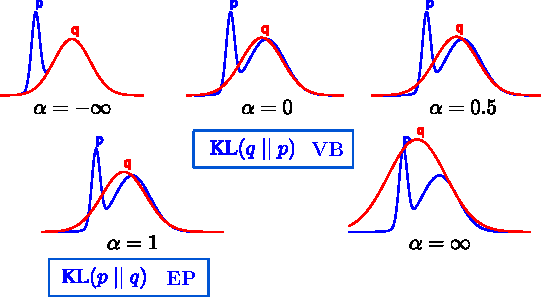
\includegraphics[width=0.7\linewidth]{Chapter3/bbalpha/figs/alpha_divergence}
 \caption{An illustration of approximating distributions by $\alpha$-divergence minimization. Here $p$ and $q$ shown in the graphs are unnormalized probability densities. Reproduced from \citet{minka:divergence2005}. Best viewed in color.}
 \label{fig:alpha_divergence}
\end{figure}

Setting aside the analytic tractability of the computations, we note that the
minimisation of a global $\alpha$-divergence might not always be desirable. If
the true posterior has many modes, then when a Gaussian approximation is deployed, a global approximation of this flavour that
is refined using $\alpha \geq 1$ will cover the modes, and can place
substantial probability in the area where the true posterior has low
probability (see the last plot in Figure \ref{fig:alpha_divergence}). 
